\documentclass[12pt,a4paper]{article}

\usepackage[utf8]{inputenc}
\usepackage[margin=2.5cm]{geometry}
\usepackage{newtxtext,newtxmath}
\usepackage{amsmath}
\usepackage{booktabs}
\usepackage{tabularx}
\usepackage{array}
\usepackage{makecell}
\usepackage{graphicx}
\usepackage{caption}
\usepackage{subcaption}
\usepackage{microtype}
\usepackage{cite}
\usepackage{setspace}
\setstretch{1.52}
\usepackage[hidelinks,colorlinks=false]{hyperref}

\captionsetup{font=small,labelfont=bf}

\title{\vspace{-1.0em}\textbf{\Large Surveillance Coverage, Clinical-Process Anchors, and Workload Constraints\\ in Machine Learning Early Warning for Sepsis: An Operational Evaluation Audit}}

\author{
    \textbf{Alireza Shayan}$^{1}$, \quad \textbf{Somayeh Afrasiabi}$^{1,*}$ \\[0.4em]
    $^{1}$Department of Computer Science and Engineering \& IT,\\
    School of Electrical and Computer Engineering, Shiraz University, Shiraz, Iran \\
    \texttt{Ali404@hafez.shirazu.ac.ir}, \quad \texttt{afrasiabi@shirazu.ac.ir} \\[0.3em]
    $^{*}$Corresponding Author: Somayeh Afrasiabi (\texttt{afrasiabi@shirazu.ac.ir})
}

\date{}

\begin{document}

\maketitle

\begin{abstract}
\noindent\textbf{Objectives:} To evaluate how surveillance coverage, clinical-process anchors, and alert workload constraints govern estimated performance and evaluability in sepsis early warning.

\vspace{0.25em}
\noindent\textbf{Materials and Methods:} We evaluated 8 predictive architectures across 8,254 first ICU stays from MIMIC-III MetaVision (2008--2012; 97,700 windows; prevalence 0.694\%) during hours 19--30. We formalized an operational cascade ($S \to V \to O \to D$), quantified order date coarsening, and evaluated alert frontiers under 12-hour alert suppression.

\vspace{0.25em}
\noindent\textbf{Results:} Among 408 operational Sepsis-3 stays ($S=1$), 257 (63.0\%) developed onset after hour 36 ($V=0$). Among 151 covered stays ($V=1$), 100 (66.2\%) were first-bin assigned ($T_{\mathrm{susp}} - T_{\mathrm{S3}} \in [24\mathrm{h}, 25\mathrm{h})$), structurally guaranteeing pre-suspicion eligibility; 50 of the remaining 51 were also eligible ($O=1$: 150/151, 99.3\%). Evaluating opportunity against earliest prescription dates under midnight assignment eliminated all horizon-positive observations (0/151 definite; bounds $[0.0\%, 31.1\%]$ covered, $[0.0\%, 11.5\%]$ cohort-wide), preventing discrimination estimation. At 10 alert episodes/100 patient-days (407 emitted alerts), BiMamba SSM and LightGBM each detected 7 patients ($D=1$), yielding episode PPV 1.72\% (7/407, NNE 58.1), covered sensitivity 4.64\% (7/151), and population yield 1.72\% (7/408).

\vspace{0.25em}
\noindent\textbf{Discussion:} Evaluability and lead-time estimates depend fundamentally on protocol coverage and process-anchor definitions.

\vspace{0.25em}
\noindent\textbf{Conclusion:} Sepsis predictive evaluations must report protocol coverage, distinguish structurally induced eligibility from biological lead time, and benchmark under explicit bedside workload constraints.

\vspace{0.25em}
\noindent\textbf{Keywords:} Sepsis Early Warning, Surveillance Truncation, Anchor Selection, Alert Budget Frontier, State-Space Models.
\end{abstract}

\section{Introduction}

\subsection{Background and Significance}
Sepsis remains a leading cause of critical illness, inpatient mortality, and healthcare expenditure globally~\cite{singer2016sepsis,seymour2016assessment}. Clinical treatment urgency depends critically on presentation: the Surviving Sepsis Campaign international guidelines recommend immediate antimicrobial therapy, ideally within one hour, for possible septic shock or a high likelihood of sepsis, while recommending rapid diagnostic assessment for possible sepsis without shock~\cite{evans2021surviving,kumar2006duration}. To support prompt intervention, the biomedical informatics community has heavily invested in machine learning (ML) models for early warning. Scores of retrospective investigations have reported high discriminative capability, frequently reporting area under the receiver operating characteristic curve (AUROC) values between 0.80 and 0.88 ahead of consensus onset~\cite{moor2021early}. However, published ICU prediction studies differ substantially in outcome implementation, temporal alignment, and evaluation design; consequently, reported AUROCs should not be interpreted as directly comparable measures of deployment readiness~\cite{moor2021early,wang2025methodological}. Prior MIMIC-III analyses have shown that alternative operational onset definitions can change measured performance as much as or more than changing model class~\cite{cohen2024subtle}. These findings motivate separating reference-event construction from surveillance coverage and alert-policy evaluation. Time-sensitive sepsis benchmarks have also incorporated utility functions that reward and penalize alerts according to their timing~\cite{reyna2020early}. Such approaches reinforce the need to report temporal evaluation rules, although benchmark utility is distinct from measured clinical benefit.

Clinical evaluations have reported heterogeneous performance and outcome associations~\cite{wong2021external,adams2022prospective}, while clinician-vignette studies have identified discrepancies between operational onset labels and recommended treatment timing~\cite{weissman2024sepsis}. External evaluation of the original Epic Sepsis Model demonstrated that reported performance depended heavily on the evaluation level and timing rules: hospitalization-level and prediction-level workload estimates were not interchangeable, emphasizing the need to report the exact unit of evaluation~\cite{wong2021external}. Prospective evaluations of early-warning systems such as TREWS have found associations between timely alert confirmation and improved outcomes among selected patients identified prior to antibiotic initiation~\cite{adams2022prospective,henry2022factors}. However, because provider response was observational rather than randomized, these findings support potential clinical utility without establishing universal causal efficacy~\cite{adams2022prospective}. 

Furthermore, ICU clinicians already encounter substantial alarm exposure from bedside physiological monitors~\cite{drew2014insights}. In other clinical decision-support settings, repeated alerts and work complexity have been associated with lower alert acceptance, supporting explicit reporting of notification burden~\cite{ancker2017effects,paine2016systematic}.

Recent evaluations of sepsis early warning before clinical intervention present divergent findings. Kamran et al.~\cite{kamran2024evaluation} reported a severe decline in Epic model AUROC (0.62 to 0.47) when excluding predictions following clinical recognition. Conversely, in a multi-center study spanning 198,494 encounters across nine hospitals, Dutta et al.~\cite{dutta2026performance} demonstrated that predictive performance was preserved under certain pre-clinical action definitions. Do et al.~\cite{do2026continuous} further showed that continuous surveillance and alert silencing rules fundamentally alter clinical workload across health systems. This literature indicates that pre-intervention performance does not follow a uniform collapse, but rather depends on how onset labels, clinical-process anchors, and evaluation units are constructed. We deliberately benchmark continuous multivariate ML models rather than traditional bedside scoring heuristics (e.g., qSOFA, NEWS2, MEWS); discrete integer scores exhibit coarse step-function behavior that prevents exact alert-budget matching without tie-breaking degradation, while $\Delta\text{SOFA}$ is endogenous to the Sepsis-3 reference outcome itself.

These findings motivate the central question of this study: \textit{Why do estimates of pre-clinical action opportunity and alert performance diverge across evaluation designs?} We show that existing evaluations must distinguish four evaluation components that may be reported jointly or incompletely:
\begin{enumerate}
    \item \textbf{Incident Target Sepsis ($S$):} True clinical onset of acute organ dysfunction meeting consensus operational criteria.
    \item \textbf{Surveillance Protocol Coverage ($V$):} Fixed observation schedules may miss episodes occurring outside the evaluated interval.
    \item \textbf{Clinical-Process Anchors and Timestamp Uncertainty ($O$):} Decision opportunities depend heavily on whether anchors are placed at clinical suspicion or recorded medication orders, and whether discrete search windows structurally induce pre-anchor separation.
    \item \textbf{Emitted-Alert Workload Constraints ($D$):} Even when discrimination is preserved, operational alert budgets and suppression rules bound real-world sensitivity and positive predictive value (PPV).
\end{enumerate}

To disentangle these mechanisms, we conducted an operational evaluation audit across 8 predictive architectures using electronic health record (EHR) data from the MIMIC-III database (v1.4; CareVue development and MetaVision evaluation replay)~\cite{johnson2016mimiciii}. Our contributions are:
\begin{enumerate}
    \item \textbf{Evaluation Audit Framework:} We formalize the four-stage operational cascade $S \to V \to O \to D$, disentangling incident target sepsis, surveillance protocol coverage, process-anchor eligibility, and emitted-alert workload constraints.
    \item \textbf{Structural Analysis of Pre-Anchor Eligibility:} We show that high pre-suspicion opportunity ($150/151$, 99.3\% without buffer; $149/151$, 98.7\% with 2h buffer) is largely driven by the discrete Sepsis-3 24h lookback window in first-bin assigned cases ($100/151$, 66.2\%; $G_i \in [24\mathrm{h}, 25\mathrm{h})$), where pre-anchor separation is algebraically guaranteed rather than reflecting unprompted biological warning.
    \item \textbf{Operational Alert-Budget Frontiers:} We benchmark 8 models under strict alert budgets (5, 10, 20 episodes/100 patient-days) with a 12-hour alert suppression rule.
    \item \textbf{Multi-Clock Timestamp Uncertainty Bounds:} We bound opportunity under order dates vs. interval bounds, showing why earliest-prescription proxies yield zero estimable positive cases under midnight assignment.
    \item \textbf{Exploratory Outcome-Stratified Sensitivity:} We evaluate discrimination on hybrid sets ($\mathcal{R}_0^{\mathrm{hybrid}}, \mathcal{R}_2^{\mathrm{hybrid}}$) as an exploratory analysis, explaining why stability reflects outcome-specific censoring rather than uniform prospective policy.
\end{enumerate}

\section{Materials and Methods}

\subsection{Study Design and Cohort Definition}
We conducted a retrospective evaluation with sequential prediction replay using the MIMIC-III critical care repository (v1.4) from BIDMC~\cite{johnson2016mimiciii}, evaluating transportability across clinical information systems from CareVue (2001--2008 development) to MetaVision (2008--2012 evaluation replay), with broad historical prescriptions providing a sensitivity analysis. Analyses used versioned extraction queries with dataset identifiers and checksums recorded in the release manifest. The study cohort was defined as adult patients ($\ge 18$ years) admitted to an intensive care unit with a total ICU length of stay $\text{LOS} \ge 30\text{h}$ to evaluate mid-stay surveillance following an initial observation period (hours 0--18). While conditioning on $\text{LOS} \ge 30\text{h}$ defines a retrospectively selected longer-stay cohort (conditional on ICU survival and stay duration $\ge 30\text{h}$), it ensures all included patients remain under observation throughout the surveillance interval unless censored. To avoid within-patient clustering across multiple admissions, only the chronological first ICU stay per patient was retained. Complete cohort derivation schemas, exclusion criteria, train/validation/test partitions, feature dictionaries, missing-data rules, model architectures, and executable Sepsis-3 definitions are detailed in the Supplementary Methods Package.

Surveillance was evaluated under a prespecified second-day ICU surveillance protocol: predictions were generated at 12 scheduled hourly decision bins $[t-1, t]$ for $t \in \{19, 20, \dots, 30\}$ hours post-admission. In prospective streaming deployment, patients would enter surveillance at hour 19 and be administratively right-censored at discharge or death. The test partition comprised 8,254 unique patient ICU stays (97,700 evaluated windows, 4,070.8 patient-days of surveillance volume). Stays were censored at Sepsis-3 onset ($N=110$ stays, 623 windows) or upon observation-availability cessation prior to hour 30 ($N=180$ control stays, 725 windows, triggered by cessation of charted vital sign telemetry in the EHR). Reporting was organized in accordance with TRIPOD+AI and STROBE recommendations~\cite{collins2024tripod,vonelm2007strobe}.

\subsection{Outcome Definition and Operational Clocks}
Sepsis was defined according to a study-specific operational adaptation of Sepsis-3 criteria~\cite{singer2016sepsis,seymour2016assessment}: an acute increase in Sequential Organ Failure Assessment (SOFA) score $\ge 2$ points over baseline. Baseline SOFA ($\text{SOFA}_{\text{base}}$) was defined in the frozen implementation as the minimum total SOFA score observed in the 24-hour window preceding the suspicion anchor ($t \in [T_{\mathrm{susp}} - 24\mathrm{h}, T_{\mathrm{susp}}]$, assumed 0 if no prior measurements existed). Sepsis-3 onset was identified when total SOFA increased by $\ge 2$ points above $\text{SOFA}_{\text{base}}$ within the clinical search window $[T_{\mathrm{susp}} - 24\text{h}, T_{\mathrm{susp}} + 12\text{h}]$ relative to suspected infection (defined as blood culture specimen collection paired with systemic antimicrobial prescription orders; detailed in Supplementary Section S1.5). In the MIMIC-III database, antimicrobial timing derives from recorded prescription scheduling dates (\texttt{prescriptions.\allowbreak startdate}), which represent medication order records rather than electronically verified bedside administration timestamps. While MetaVision records minute-resolved intravenous infusions in \texttt{inputevents\_mv} (and MIMIC-IV provides barcode-verified \texttt{emar} logs), we audit the date-coarsened \texttt{prescriptions} table because it reflects standard practice across published benchmarks, maintains CareVue compatibility, and captures pre-ICU ward and oral orders that precede ICU admission.

To resolve temporal precision and event ambiguity without conflating orders, intended start dates, and physical administrations, we track six operational milestones (with ICU admission as the reference origin $t=0$, followed by five operational event clocks; Figure~\ref{fig:clocks}):
\begin{itemize}
    \item $T_{\text{admit}, i}$: ICU admission timestamp ($t=0$, reference origin).
    \item $T_{\mathrm{Rx,start}, i}$: Earliest documented systemic antimicrobial prescription start date (\texttt{prescriptions}\allowbreak\texttt{.startdate}, calendar date coarsened to midnight 00:00:00).
    \item $T_{\mathrm{abx,pair}, i}$: Systemic antimicrobial order date participating in the qualifying infection suspicion pair.
    \item $T_{\mathrm{culture,pair}, i}$: Blood culture specimen collection timestamp (\texttt{microbiology}\allowbreak\texttt{events.charttime}, minute-level precision).
    \item $T_{\mathrm{susp}, i}$: Operational infection-suspicion anchor, defined per Seymour et al.~\cite{seymour2016assessment} as $\min(T_{\mathrm{abx,pair}},$ $T_{\mathrm{culture,pair}})$.
    \item $T_{\text{S3}, i}$: Operationally assigned Sepsis-3 onset timestamp.
\end{itemize}

When blood culture precedes antimicrobial prescription ($T_{\mathrm{culture,pair}} < T_{\mathrm{abx,pair}}$), $T_{\mathrm{susp}} = T_{\mathrm{culture,pair}} \ne T_{\mathrm{abx,pair}}$. Let $h = 1\text{ h}$ and define the dimensionless lookback coordinate $x_i = (T_{\mathrm{susp}, i} - 24\text{h} - T_{\text{admit}, i})/h$. The search window evaluates discrete hourly bins starting at $\texttt{baseline\_start\_h}_i = \lfloor x_i \rfloor$ and ending at $\texttt{window\_end\_h}_i = \lfloor(T_{\mathrm{susp}, i} + 12\text{h} - T_{\text{admit}, i})/h\rfloor$. Because the upper boundary bin is floored, evaluated hours never exceed $T_{\mathrm{susp}} + 12\text{h}$, strictly guaranteeing $T_{\mathrm{susp}, i} - T_{\text{S3}, i} \ge -12.0\text{h}$ (empirical minimum: $-11.2\text{h}$). For episodes where acute $\Delta\text{SOFA} \ge 2$ is first observed at the earliest search bin ($N=274/408$, 67.2\% of all incident sepsis; and $100/151$, 66.2\% of surveillance-covered stays), onset is assigned as $T_{\text{S3}, i} = T_{\text{admit}, i} + h\lfloor x_i \rfloor$, yielding the operational lead gap:
\begin{equation}
G_i = T_{\mathrm{susp}, i} - T_{\text{S3}, i} = 24\text{h} + h\,\operatorname{frac}(x_i)
\end{equation}
Because $0 \le \operatorname{frac}(x_i) < 1$ (dimensionless), first-bin-assigned episodes satisfy $24\text{h} \le G_i < 25\text{h}$, with an analytical supremum of $25\text{h}$ (the reported $24.99\text{h}$ is the observed empirical maximum). In these first-bin episodes ($100/151$, 66.2\% of surveillance-covered stays), pre-suspicion opportunity ($t < T_{\mathrm{susp}}$) is algebraically guaranteed for any decision time evaluated prior to onset ($t < T_{\mathrm{S3}} \approx T_{\mathrm{susp}} - 24\text{h}$), and the 2-hour buffer is trivially satisfied (100/100 eligible under both $\delta=0\mathrm{h}$ and $\delta=2\mathrm{h}$). For the remaining 51 non-first-bin covered stays (33.8\%), the median lead gap was 19.3\text{h} (IQR: 7.1--22.0\text{h}; 45 of 51 exhibiting $T_{\mathrm{susp}} > T_{\mathrm{S3}}$). Because evaluated early-warning decisions occur up to 6\text{h} prior to onset ($t < T_{\mathrm{S3}}$), pre-suspicion opportunity holds for 50 of the 51 non-first-bin stays under $\delta=0\mathrm{h}$ (1 ineligible stay, detailed in Supplementary Audit Table) and 49 of 51 under $\delta=2\mathrm{h}$ (2 ineligible stays). Across all 151 covered stays, pre-suspicion eligibility is thus $100 + 50 = 150/151$ (99.3\%) under $\delta=0\mathrm{h}$ and $100 + 49 = 149/151$ (98.7\%) under $\delta=2\mathrm{h}$. Thus, high pre-suspicion opportunity in Sepsis-3 largely reflects the discrete lookback convention rather than independent empirical evidence of unprompted biological warning. Across the full 408 cohort, the median lead gap was $+24.2\text{h}$ (IQR: $22.8\text{h}$ to $24.6\text{h}$; range: $-11.2\text{h}$ to $+24.99\text{h}$).

\begin{figure}[t]
    \centering
    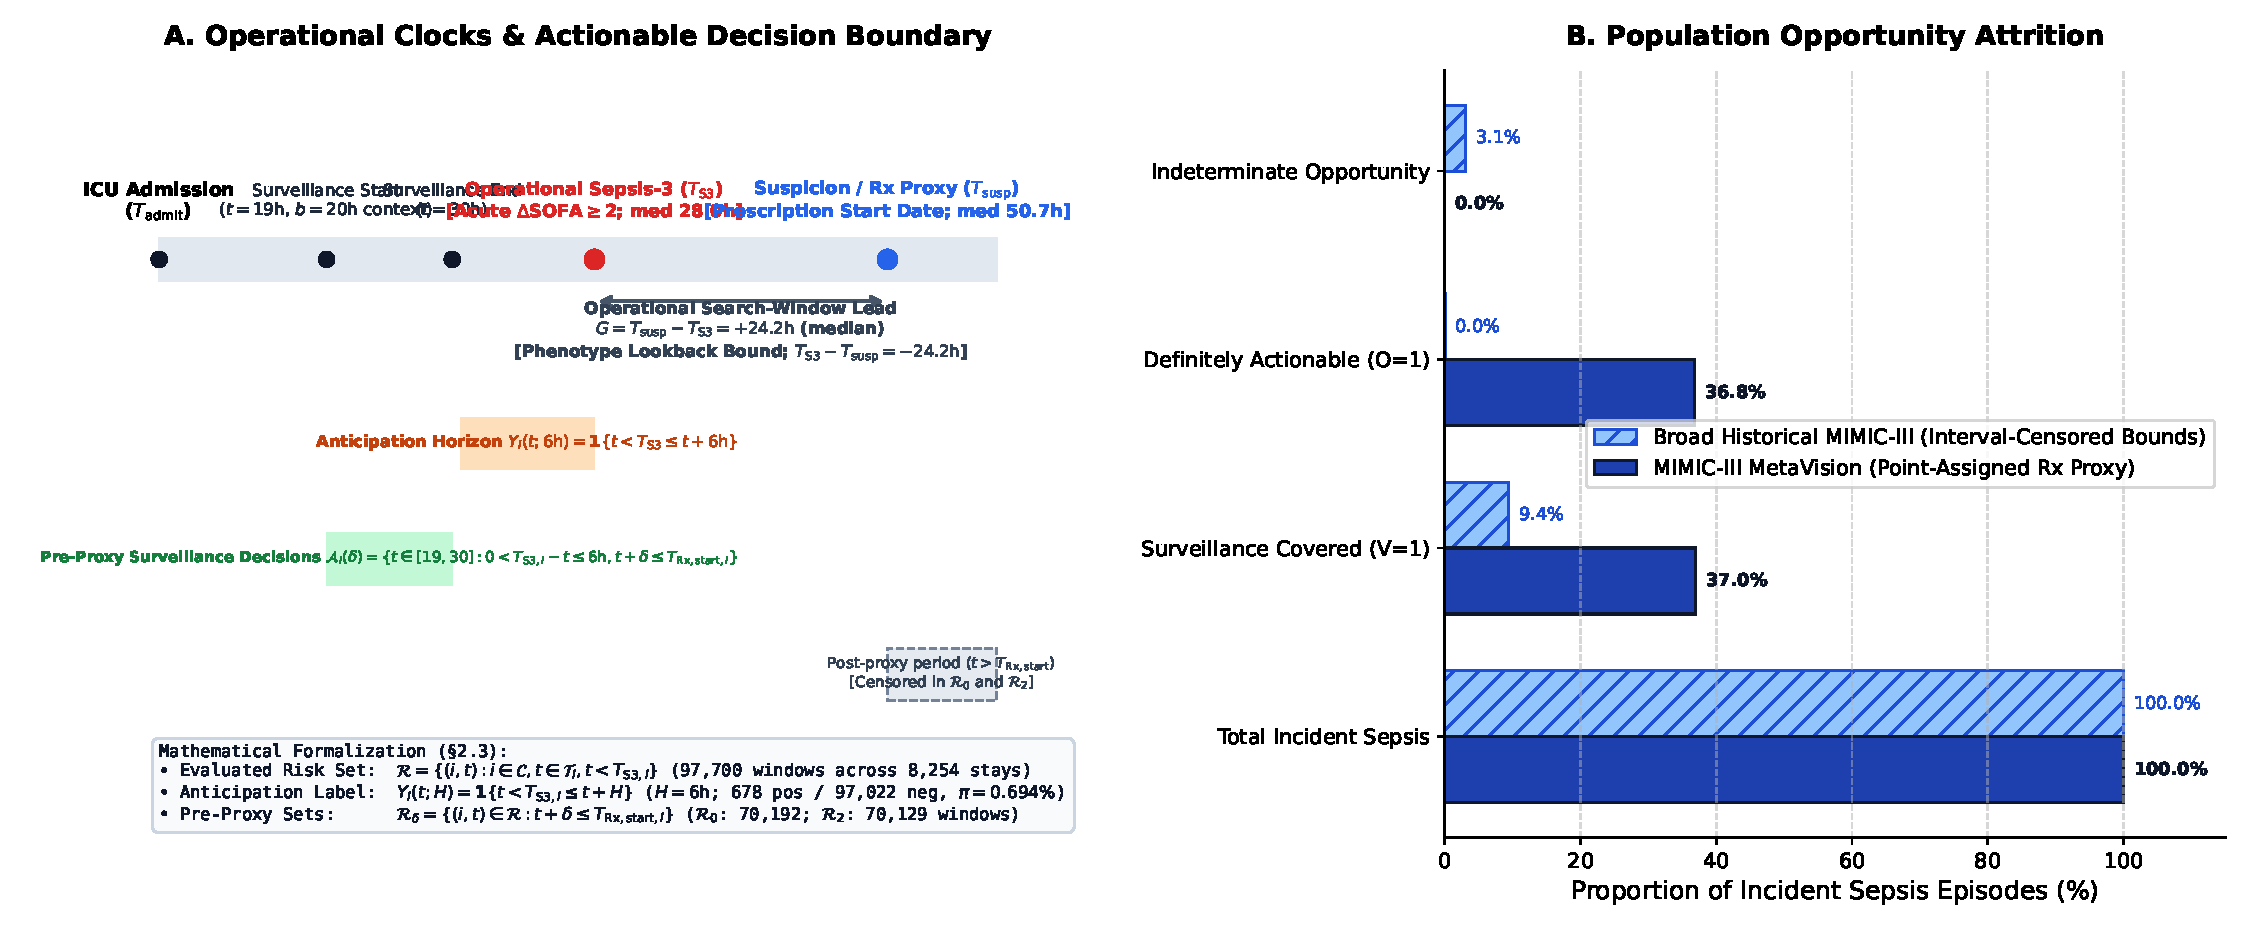
\includegraphics[width=0.92\textwidth]{figures/Figure1_Clocks_and_Opportunity_Waterfall.pdf}
    \caption{\textbf{Operational Clocks and Anchor-Dependent Evaluation Eligibility in the MIMIC-III MetaVision Cohort.} The timeline is schematic; displayed population summaries do not represent a single paired patient trajectory. Eligibility relative to a retrospective suspicion anchor does not establish absence of prior antimicrobial exposure. Panel A depicts the clinical timeline for an ICU-incident sepsis stay, illustrating the discrete search-window lead $G_i = 24\text{h} + h\,\operatorname{frac}(x_i) < 25\text{h}$ for first-bin-assigned episodes ($N=274/408$, 67.2\%; median $+24.2\text{h}$; empirical max $24.99\text{h}$), the anticipation horizon $t \in [22\mathrm{h}, 28\mathrm{h})$, anchor-eligible decision times $\mathcal{A}_i^{(C)}(\delta)$, and the conceptual post-anchor period. Actual model evaluations occur at discrete scored timestamps $t \in \mathcal{T}_i$. Panel B displays population opportunity attrition comparing Broad Historical MIMIC-III (earliest prescription proxy $T_{\mathrm{Rx,start}}$, $N=3,581$) and MIMIC-III MetaVision (suspicion anchor $T_{\mathrm{susp}}$, $N=408$), reporting exact stay counts beside each opportunity tier under declared midnight assignment. \textit{Alt-text:} Two-panel diagram displaying schematic timeline clocks and formal risk-set definitions in Panel A, and horizontal bar charts comparing surveillance coverage and treatment-precedence opportunity in Panel B.}
    \label{fig:clocks}
\end{figure}

\subsection{Operational Cascade and Outcome-Stratified Hybrid Risk Sets}
Let $\mathcal{C}$ denote the evaluated test cohort of unique ICU stays ($N = 8,254$), and let $\mathcal{T}_i \subseteq \{19, 20, \dots, 30\}$ denote the set of hourly decision bins evaluated for stay $i$. For patients who never develop operational Sepsis-3 during hospitalization, we set $T_{\text{S3}, i} = \infty$.

The full evaluated early-warning risk set is defined as:
\begin{equation}
\mathcal{R} = \bigl\{ (i, t) : i \in \mathcal{C}, \; t \in \mathcal{T}_i, \; t < T_{\text{S3}, i} \bigr\}
\end{equation}
The binary early-warning prediction target at anticipation horizon $H = 6\text{h}$ is:
\begin{equation}
Y_i(t; H) = \mathbf{1} \bigl\{ t < T_{\text{S3}, i} \le t + H \bigr\}
\end{equation}
In the canonical unconstrained risk set ($\mathcal{R}_{\text{canonical}} = \mathcal{R}$), this definition yields exactly 97,700 evaluated hourly windows, comprising 678 horizon-positive observations ($Y=1$) and 97,022 negative observations ($Y=0$, prevalence $\pi = 0.694\%$).

The four stages of the operational cascade ($S \to V \to O \to D$) are formalized via stay-level indicators: $S_i = \mathbf{1} \{ T_{\text{S3}, i} < \infty \}$, $V_i = \mathbf{1} \{ \exists t \in \mathcal{T}_i : Y_i(t; 6\text{h}) = 1 \}$, $O_i(\delta) = \mathbf{1} \{ \exists t \in \mathcal{T}_i : Y_i(t; 6\text{h}) = 1 \land t + \delta \le C_i \}$, and $D_i(q) = \mathbf{1} \{ i \in \mathcal{S}_{\text{alerted}}(K) \land Y_i(t_{\mathrm{first}, i}; 6\text{h}) = 1 \land t_{\mathrm{first}, i} + \delta \le C_i \}$.

To evaluate restricted decision windows, we define the outcome-stratified hybrid risk sets relative to reference clock $C_i$:
\begin{equation}
\mathcal{R}_\delta^{\mathrm{hybrid}} = \bigl\{ (i, t) \in \mathcal{R} : t + \delta \le C_i \bigr\}
\end{equation}
where $C_i = T_{\mathrm{susp}, i} = \min(T_{\mathrm{culture,pair}, i}, T_{\mathrm{abx,pair}, i})$ for incident sepsis stays ($S_i=1$; determined by $T_{\mathrm{abx,pair}}$ in 399 stays and blood culture charttime in 9 stays), and $C_i = T_{\mathrm{Rx,start}, i}$ for non-sepsis control stays ($S_i=0$) if systemic antimicrobials were ordered during hospitalization ($C_i = \infty$ otherwise). Exactly 2,287 control stays had $T_{\mathrm{Rx,start}} \le 19\text{h}$, censoring all their windows ($W_{\mathrm{fully\ excluded}} = 27,388$). Among 83 later-prescription control stays ($T_{\mathrm{Rx,start}} > 19\text{h}$, of which 21 intersect the surveillance interval $[19, 30]\text{h}$ and 62 follow hour 30), 113 windows were censored post-prescription at $\delta=0\text{h}$ ($65,926 = 93,427 - 27,388 - 113$), and 49 additional windows were removed by the 2-hour proxy-timing margin ($65,877 = 65,926 - 49$). Together with 4,266 sepsis case windows (674 positive, 3,592 negative; 7 windows censored relative to canonical 4,273), $\mathcal{R}_0^{\mathrm{hybrid}}$ evaluates 70,192 windows across 5,967 stays (prevalence 0.960\%). At $\delta=2\text{h}$, $\mathcal{R}_2^{\mathrm{hybrid}}$ evaluates 70,129 windows (4,252 case windows; 21 censored; prevalence 0.945\%).

Importantly, sepsis cases and controls were restricted using different clinical-process anchors. Differences from canonical discrimination therefore reflect both changes in the evaluated observations and the outcome-specific selection rule; they are not estimates of performance under a uniform prospective eligibility policy. Crucially, in the uniform earliest-prescription sets ($\mathcal{R}_0^{\mathrm{Rx}}$ and $\mathcal{R}_2^{\mathrm{Rx}}$), all 408 incident sepsis stays had documented prescription start dates prior to hour 3.83 of ICU admission (median $-12.6\text{h}$, range $-23.9\text{h}$ to $+3.83\text{h}$) due to midnight date-coarsening; consequently, all 4,273 case windows (including all 678 positive windows, all 511 baseline negative windows from covered stays, and all 3,084 negative windows from late-onset stays) were excluded as post-prescription ($t \ge 19.0\text{h} > T_{\mathrm{Rx,start}}$). The surviving 65,926 windows in $\mathcal{R}_0^{\mathrm{Rx}}$ (and 65,877 in $\mathcal{R}_2^{\mathrm{Rx}}$) originate exclusively from non-sepsis controls ($N=5,559$). Because no horizon-positive cases remained ($N_+^{\mathrm{Rx}} = 0$; prevalence strictly 0.000\%), discrimination was mathematically unestimable: AUROC is undefined and AUPRC yields an uninformative point estimate.

\subsection{Alert-Budget Operating Frontiers and Refractory Policy}
To evaluate operational bedside burden, we benchmark alert budgets $q \in \{5.0, 10.0, 20.0\}$ emitted alert episodes per 100 surveillance patient-days. For exposure $E = \frac{1}{24}\sum_{i\in\mathcal{C}} |\mathcal{T}_i|$ patient-days (where $h_i = |\mathcal{T}_i|$ is the number of evaluated hourly windows for stay $i$; $E=4,070.8$ pt-days in the test cohort), the allowed alert episode quota is $K = \operatorname{round}(q \cdot E / 100)$, yielding exactly $K \in \{204, 407, 814\}$ alert episodes at $q \in \{5.0, 10.0, 20.0\}$. Under a 12-hour suppression rule, each stay emits at most one alert episode within the evaluated 12-hour interval ($N_{\text{episodes}, i} \le 1$). We report three operational metrics: $\text{Episode PPV} = N_{\text{det}} / N_{\text{emitted}}$, $\text{Covered Sensitivity} = N_{\text{det}} / 151$, and $\text{Population Yield} = N_{\text{det}} / 408$, where timely detections are defined as:
\begin{equation}
N_{\text{det}} = \sum_{i \in \mathcal{S}_{\text{alerted}}(K)} \mathbf{1} \{ S_i = 1 \land Y_i(t_{\mathrm{first}, i}; 6\text{h}) = 1 \land t_{\mathrm{first}, i} + \delta \le C_i \}
\end{equation}
Candidate alert selection is performed across the full canonical stream $\mathcal{R}$. Under the 12-hour refractory rule, each patient emits at most one alert across the 12-hour surveillance window; this policy is mathematically equivalent to ranking patients by their maximum predicted risk score $\max_{t \in \mathcal{T}_i} s_i(t)$. The operating threshold $\tau(K) = \min_{j \in \mathcal{S}_{\text{alerted}}(K)} \max_{t \in \mathcal{T}_j} s_j(t)$ is defined by the peak score of the $K$-th ranked patient. Candidate alert selection is governed by $\mathcal{B} = (q, E, K)$, and ties at the operating threshold are deterministically resolved by $\mathcal{S}_{\text{alerted}}(K)$, defined as the top $K$ patient replicas under the lexicographical order $(-\max_{t} s_i(t), \;\text{ICUSTAY\_ID}, \;\text{copy\_idx})$, where $\text{copy\_idx}$ indexes duplicated instances under bootstrap resampling. Detection timing is evaluated at the first threshold crossing: $t_{\mathrm{first}, i} = \min \{ t \in \mathcal{T}_i : \operatorname{Elig}_i(t; \tau, \mathcal{B}) = 1 \}$, where $\operatorname{Elig}_i(t; \tau, \mathcal{B}) = \mathbf{1} \{ i \in \mathcal{S}_{\text{alerted}}(K) \land s_i(t) \ge \tau \}$.

\subsection{Predictive Models and Statistical Inference}
We evaluated 8 models spanning three major architectural paradigms: (1) State-Space Models (BiMamba SSM)~\cite{gu2023mamba,gu2022efficiently}; (2) Deep Sequence Transformers (Mask-Aware Clinical Transformer and Baseline Unmasked Transformer); (3) Tabular and Ensemble Baselines (Random Forest, XGBoost, LightGBM, L2 Logistic Regression, and Multi-Model Stacking Ensemble). Models consumed a causal 20-hour observation lookback $[t-20\text{h}, t)$ across 21 physiological time series. For tabular models (GBDTs, Random Forest, Logistic Regression), the $20 \times 21$ hourly matrix was flattened into a 420-dimensional feature vector. The Stacking Ensemble combined out-of-fold cross-validated predictions across all five base learners using an L2 logistic meta-learner. At $t=19\text{h}$, the pre-admission bin $[-1\text{h}, 0\text{h})$ was zero-masked, and BiMamba SSM bidirectional selective scans were computed within each 20-hour slice with linear $O(L)$ scan complexity and mean sequence pooling over time steps. We intentionally delimited the audit scope to continuous multivariate ML models and excluded traditional bedside scoring heuristics (e.g., qSOFA, NEWS2, MEWS, $\Delta\text{SOFA}$): discrete integer scores have coarse step-function distributions with heavy ties that preclude smooth alert-budget thresholding, while $\Delta\text{SOFA}$ is endogenous to the Sepsis-3 definition itself.

Uncertainty was quantified using patient-clustered paired bootstrapping ($B=1,000$ resamples). For Procedure B (Empirical Burden-Matched Bootstrap), exposure $E_b = \frac{1}{24}\sum_{i\in b} h_i$ and alert target $K_b = \operatorname{round}(q \cdot E_b / 100)$ were dynamically recomputed within each resample. NNE confidence intervals were derived by exact reciprocal transformation from unrounded $\text{PPV}_b$: $\text{NNE}_{\text{low}} = 100 / \text{PPV}_{\text{upper}}$ and $\text{NNE}_{\text{high}} = 100 / \text{PPV}_{\text{low}}$ ($+\infty$ when $\text{PPV}_{\text{low}} = 0$).

\section{Results}

\subsection{Cohort Progression and Denominator Accounting}
Table~\ref{tab:table1} traces all 8,254 ICU admissions through surveillance eligibility, onset timing, lookback horizons, and pre-treatment actionability. Across all 408 operational Sepsis-3 stays, median onset was 49.0h post-admission. Exactly 257 stays (63.0\%; median onset: 69.0h) had clinical onset after hour 36. Under the specified observation schedule and 6-hour horizon, these 257 stays had no evaluated horizon-positive decision time ($V=0$). The remaining 151 stays (37.0\%; median onset: 28.0h) had active protocol surveillance coverage ($V=1$). Of the 151 covered stays, 150 had at least one horizon-positive decision time at or before the selected infection-suspicion anchor (99.3\% within-covered opportunity; 36.8\% of total incident sepsis under $\delta=0\mathrm{h}$; and 149 stays, 98.7\% under $\delta=2\mathrm{h}$).



\subsection{Outcome-Stratified Hybrid Discrimination Analysis}
Table~\ref{tab:table2} presents discrimination across Canonical Sepsis-3, Hybrid Set ($\mathcal{R}_0^{\mathrm{hybrid}}$), and Hybrid Set with 2h Buffer ($\mathcal{R}_2^{\mathrm{hybrid}}$). Discrimination changed little in the outcome-stratified hybrid analysis (BiMamba SSM: AUROC 0.6326 canonical vs. 0.6433 on $\mathcal{R}_0^{\mathrm{hybrid}}$, paired $\Delta\text{AUROC} = +0.0107$, 95\% CI: +0.0060 to +0.0175; Stacking Ensemble: 0.6284 vs. 0.6351, paired $\Delta\text{AUROC} = +0.0067$). Because cases and controls were restricted using different anchors, this finding does not establish preserved discrimination under a uniform pre-suspicion or pre-prescription policy. The increase in raw AUPRC (BiMamba: 1.209\% to 1.656\%) was mechanically driven by control-window censoring, which raised baseline positive prevalence by $1.384\times$ (from $\pi=0.694\%$ to $0.960\%$). When evaluated as prevalence-normalized lift ($\text{AUPRC}/\pi$), discriminative gain over baseline remains essentially flat ($1.742\times$ canonical vs. $1.725\times$ on $\mathcal{R}_0^{\mathrm{hybrid}}$ for BiMamba, and $1.738\times$ vs. $1.688\times$ for the Stacking Ensemble), confirming that raw AUPRC increases reflect control-window denominator reduction rather than improved precision-recall ranking. These results are directionally consistent with the order-based sensitivity findings of Dutta et al.~\cite{dutta2026performance}.

\subsection{Observed Burden--Detection Trade-Off Under This Protocol}
Table~\ref{tab:table3} and Figure~\ref{fig:frontiers} demonstrate the observed trade-off under the prespecified alert-budget scenarios: bedside detection yield is constrained by alert-rate limits. Alerts were selected across the full canonical surveillance stream (4,070.8 patient-days; 97,700 windows across all 8,254 test stays); $C_i$ was used only retrospectively to adjudicate advance-warning timing ($t_{\mathrm{first}, i} + \delta \le T_{\mathrm{susp}, i}$ for sepsis cases), rather than excluding observations prior to alert selection. Retaining control stays with prior antimicrobial orders in the alert pool simulates an unconstrained clinical screening deployment; in live practice, suppressing alerts on patients already receiving broad-spectrum antimicrobials would be an operational deployment option that prevents treated controls from consuming alert capacity.

At an emitted workload of 10 alert episodes per 100 patient-days (407 emitted episodes across 4,070.8 patient-days):
\begin{itemize}
    \item Across all 8 models, episode-level PPV ranged from 0.98\% to 1.72\%, corresponding to 58.1 to 101.8 simulated evaluations per detected patient ($\text{NNE}$).
    \item BiMamba SSM and LightGBM each uniquely detected \textbf{7 patients} (PPV = 1.72\%, 95\% CI: 0.49\%--2.95\%; NNE = 58.1, 95\% CI: 33.9--203.5; covered sensitivity 4.64\%; population yield 1.72\%).
    \item Stacking Ensemble, XGBoost, and Random Forest each detected \textbf{6 patients} (PPV = 1.47\%, NNE = 67.8).
    \item Of the 407 emitted alerts for BiMamba SSM, 54 fired on sepsis stays (7 true detections within $(0, 6]\text{h}$ of onset; 47 premature or late alerts) and 353 fired on control stays. Crucially, 71 of these control alerts (17.4\% of all 407 alerts; 20.1\% of control alerts) fired on pre-treated controls ($T_{\mathrm{Rx,start}} \le 19\text{h}$), while 277 alerts (68.1\% of all alerts) fired on untreated controls, and 5 alerts on controls with prescriptions after hour 30. Across models, pre-treated controls consumed 17.4\% (BiMamba SSM, Stacking Ensemble) to 31.4\% (LightGBM; 128/407) of alert capacity. Suppressing alerts on patients already on broad-spectrum antimicrobials would eliminate 17.4\%--31.4\% of bedside false alarms without reducing true sepsis detections.
    \item In this observed evaluation, the count of horizon-correct emitted alerts and alerts additionally satisfying the two-hour pre-suspicion margin ($t_{\mathrm{first}, i} + 2\text{h} \le T_{\mathrm{susp}, i}$) were identical across all models (7 of 7 for BiMamba SSM; $N_{\mathrm{det}} = N_{\mathrm{det}, \mathrm{pre\text{-}susp}}$). These detections occurred before the suspicion anchor ($T_{\mathrm{susp}}$), not necessarily before earliest antimicrobial prescribing ($T_{\mathrm{Rx,start}}$).
    \item Model rankings varied across budgets: at 20 episodes/100 pt-days, XGBoost detected 15 patients (NNE = 54.3) and Mask-Aware Transformer detected 14 patients (NNE = 58.1).
\end{itemize}

\begin{figure}[t]
    \centering
    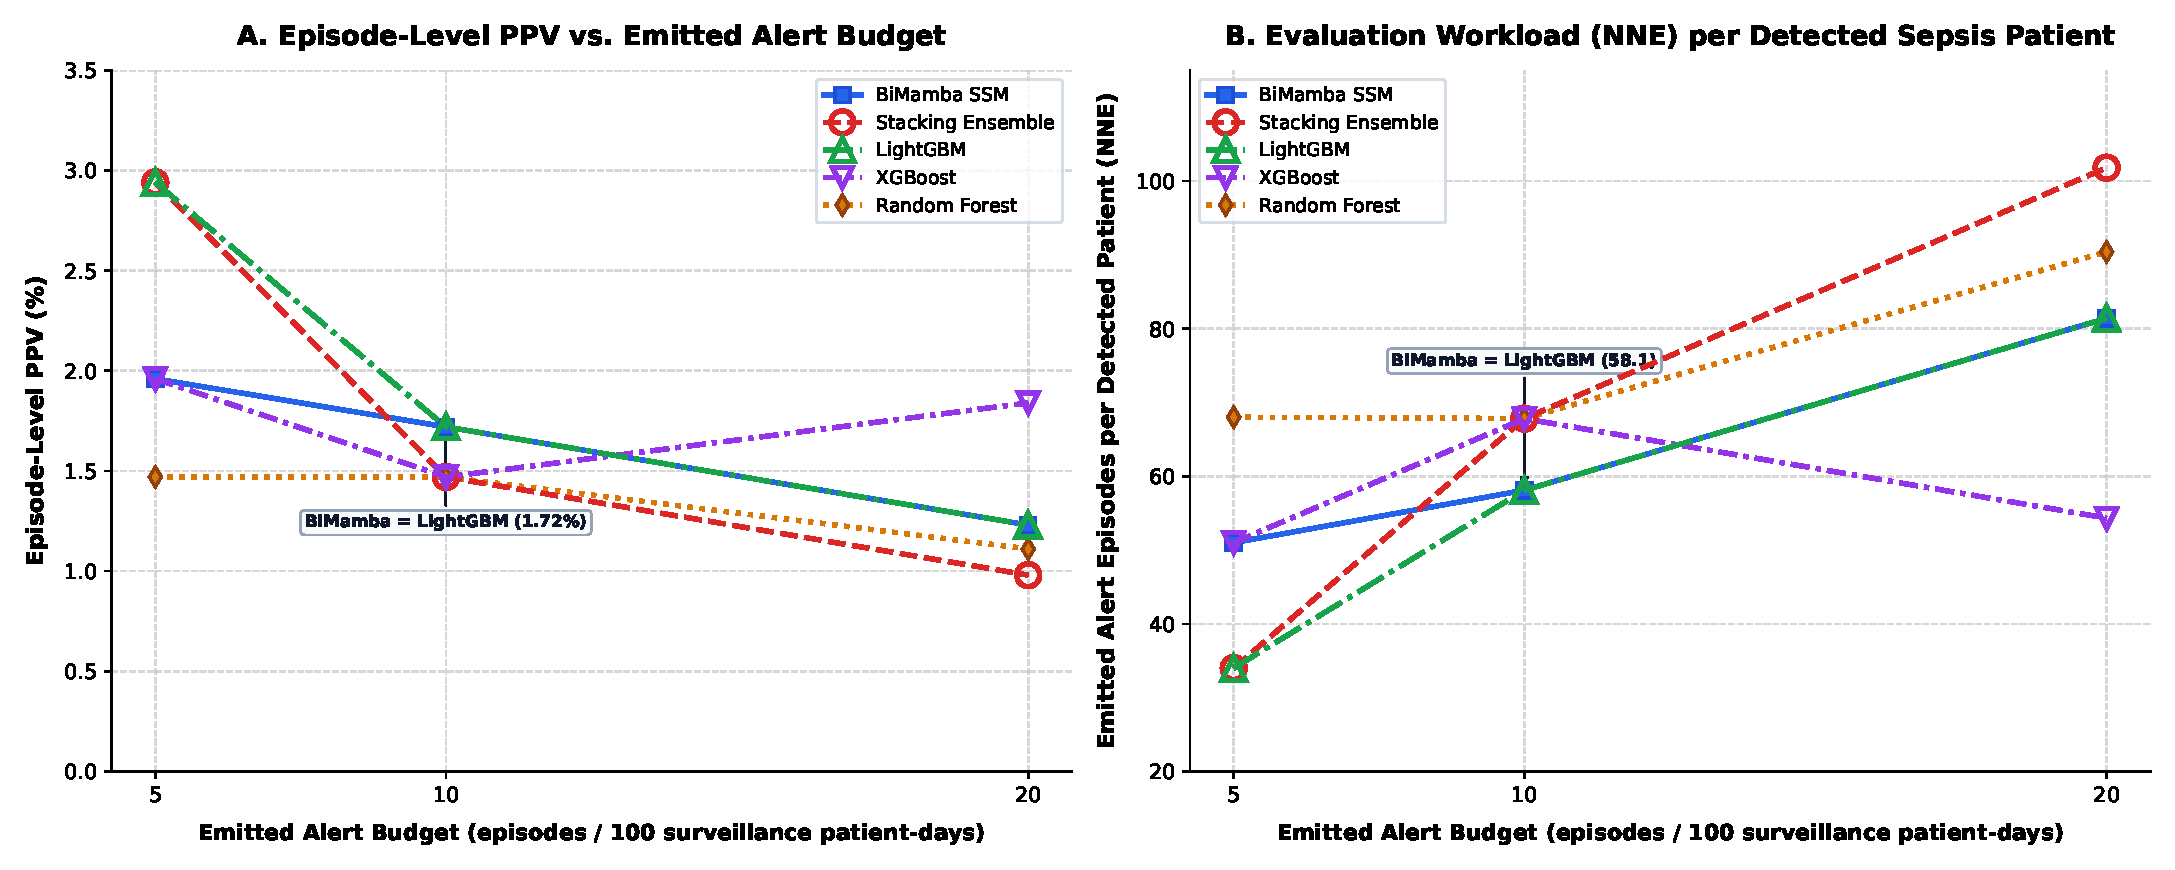
\includegraphics[width=0.90\textwidth]{figures/Figure2_Operational_Alert_Budget_Frontier.pdf}
    \caption{\textbf{Operational Alert-Budget Performance Frontier.} Panel A displays episode-level positive predictive value (PPV \%) across prespecified alert budgets. Panel B displays the Number Needed to Evaluate (NNE) per detected patient under a 12-hour alert suppression rule. Lines connect discrete prespecified operating budgets (5, 10, and 20 emitted episodes per 100 patient-days) for a representative 5-model subset; complete 8-model results, bootstrap confidence intervals, and boundary-degenerate notes are reported in Table~\ref{tab:table3}. BiMamba SSM and LightGBM have coincident operating points at budgets of 10 and 20 episodes per 100 surveillance patient-days. \textit{Alt-text:} Two-panel plot showing positive predictive value (Panel A) and evaluation workload per detected patient (Panel B) across emitted alert budgets of 5, 10, and 20 episodes per 100 patient-days for five machine learning models under 12-hour alert suppression.}
    \label{fig:frontiers}
\end{figure}

\subsection{Two-Axis Subgroup and Timestamp Uncertainty Matrix}
Table~\ref{tab:table4} presents the cross-tabulation of Sepsis Onset Timing against Treatment Proxy Timing. Because MIMIC-III prescription start dates (\texttt{prescriptions.\allowbreak startdate}) lack time of day, order initiation is evaluated both under declared point assignment (midnight $a_i$) and under calendar-day intervals $[a_i, b_i) = [\text{midnight}, \text{next midnight})$.

Opportunity depended strongly on the selected clinical-process anchor. Under the primary benchmark evaluating decision opportunity relative to the infection-suspicion anchor ($T_{\mathrm{susp}}$), 150 of 151 covered patients (99.3\% within-covered; 36.8\% of total incident sepsis) had decision bins preceding $T_{\mathrm{susp}}$ under declared midnight point assignment $a_i$. Because $a_i \le T_{\mathrm{susp}, i}$ across $[a_i, b_i)$, these 150 stays are definitely eligible throughout the calendar-day interval ($O_i^{\mathrm{def}} = 150$), with only 1 indeterminate stay ($O_i^{\mathrm{indet}} = 1$), bounding opportunity between 36.8\% and 37.0\% ($[150, 151]/408$; $[99.3\%, 100.0\%]$ within-covered). All indicators strictly satisfy $O_i^{\mathrm{def}} \le O_i^{\mathrm{point}} \le O_i^{\mathrm{poss}}$ and $O_i^{\mathrm{poss}} = O_i^{\mathrm{def}} + O_i^{\mathrm{indet}}$.

In contrast, opportunity was substantially lower and uncertain relative to the earliest hospital prescription-start proxy ($T_{\mathrm{Rx,start}}$): exactly 0 covered stays had definite opportunity under midnight point-assignment ($O_i^{\mathrm{def}} = 0, O_i^{\mathrm{point}} = 0$), with 47 indeterminate stays ($O_i^{\mathrm{indet}} = 47$), establishing bounds $[0.0\%, 11.5\%]$ ($[0, 47]/408$; $[0.0\%, 31.1\%]$ within-covered). Because no horizon-positive cases remained before point-assigned earliest prescriptions, this task was not evaluable for discrimination under midnight point assignment. In broad historical MIMIC-III ($N=3,581$), intervals generate 1 definitely eligible stay, 110 indeterminate stays, and bounds $[0.03\%, 3.10\%]$. The 150/151 result under $T_{\mathrm{susp}}$ does not establish that patients were unexposed to antimicrobials or that models predicted prior to first administration. Equally, zero definite opportunity under $T_{\mathrm{Rx,start}}$ reflects date coarsening, not verified bedside exposure.

\subsection{Cumulative Population Coverage Decomposition}
Figure~\ref{fig:decomp} illustrates the four-stage cumulative population coverage decomposition ($S \to V \to O \to D$):
\[
\frac{|V=1|}{|S=1|} \times \frac{|O=1|}{|V=1|} \times \frac{|D=1|}{|O=1|} = \frac{151}{408} \times \frac{150}{151} \times \frac{7}{150} = \frac{7}{408} = 1.72\%
\]
\begin{enumerate}
    \item \textbf{Surveillance Truncation ($151/408 = 37.0\%$):} 63.0\% of sepsis patients develop onset after hour 36, outside the prespecified second-day surveillance protocol.
    \item \textbf{Suspicion-Anchor Eligibility ($150/151 = 99.3\%$):} Of the 151 covered stays, 150 had at least one horizon-positive decision time at or before the retrospective suspicion anchor ($T_{\mathrm{susp}}$) [149 of 151 (98.7\%) under a 2-hour pre-suspicion margin].
    \item \textbf{Model-Alert Policy Detection ($7/150 = 4.67\%$):} Under an operational alert policy combining score ranking, a 10 episodes/100 patient-days budget, and a 12-hour alert suppression rule, BiMamba SSM detects 7 patients (4.67\% anchor-eligible yield, $7/151 = 4.64\%$ covered sensitivity, 1.72\% whole-population yield; NNE = 58.1).
\end{enumerate}

\begin{figure}[t]
    \centering
    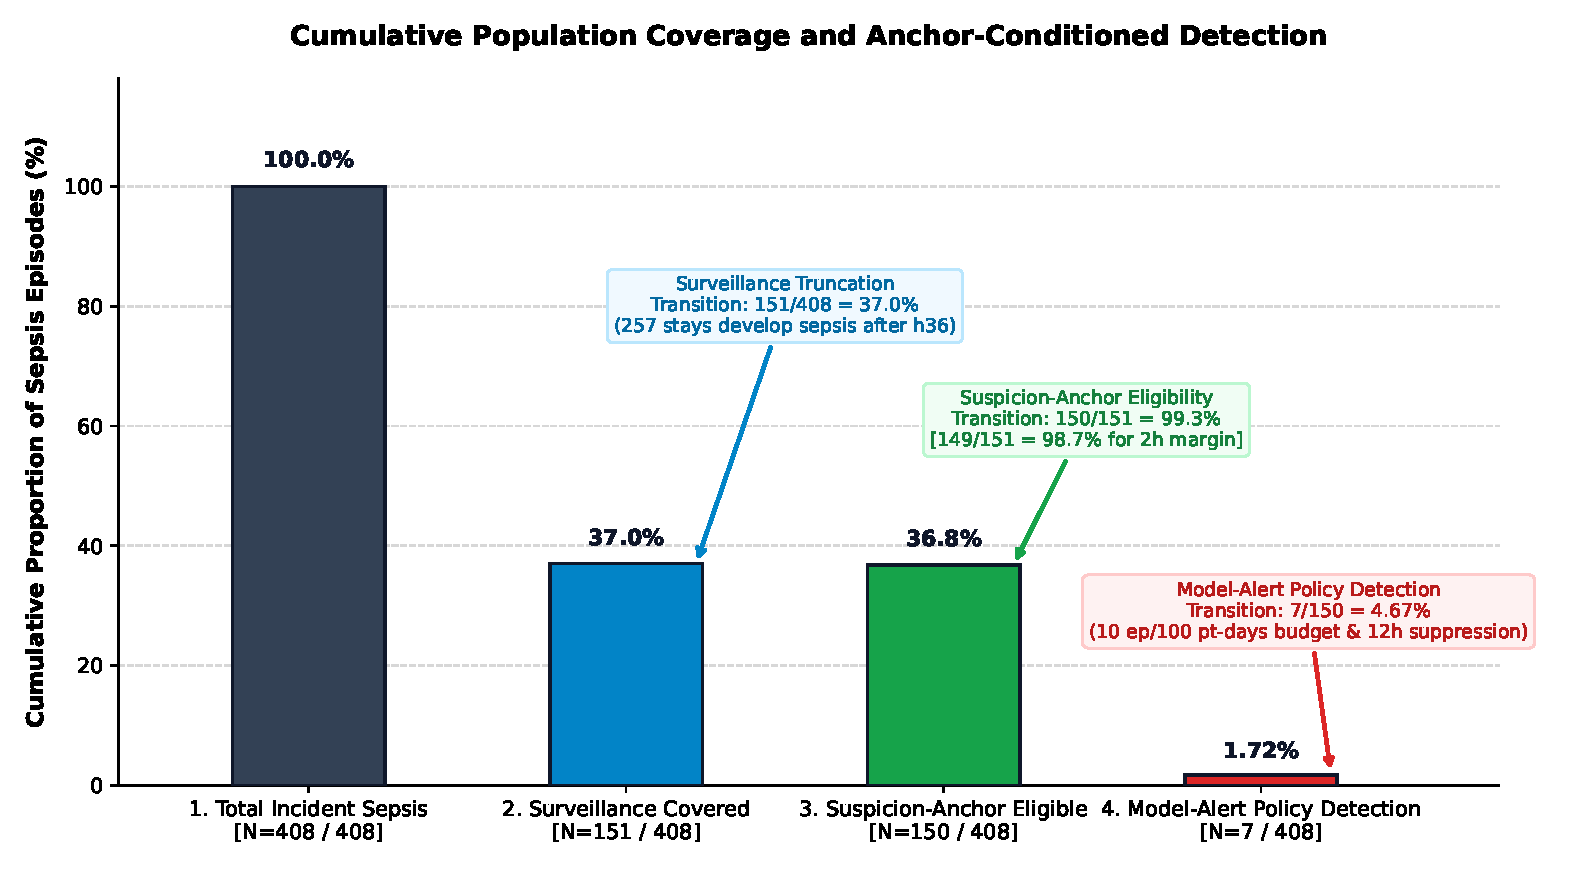
\includegraphics[width=0.88\textwidth]{figures/Figure3_Three_Stage_Decomposition.pdf}
    \caption{\textbf{Cumulative Population Coverage and Anchor-Conditioned Detection.} Stepwise attrition from 408 incident sepsis episodes through surveillance protocol coverage, retrospective suspicion-anchor eligibility, and model-alert policy detection. \textit{Alt-text:} Four-stage bar chart showing patient opportunity attrition from total incident sepsis (408 patients) to surveillance coverage (151 patients, 37.0\%), suspicion-anchor eligibility (150 patients, 36.8\%), and timely model-alert policy detection (7 patients, 1.72\%).}
    \label{fig:decomp}
\end{figure}

\section{Discussion}
This investigation characterizes the operational trade-offs governing machine learning early warning for sepsis in ICU surveillance:
\begin{enumerate}
    \item \textbf{Outcome-Dependent Anchor Selection Governs Evaluability:} The canonical surveillance analysis quantified population coverage and emitted-alert yield. A secondary outcome-stratified hybrid restriction produced small changes in discrimination, but did not represent a uniform prospective eligibility policy. Under a common earliest-prescription-start proxy and declared midnight assignment, no eligible horizon-positive observations remained, preventing discrimination estimation for that restricted task.
    \item \textbf{Detection Yield Is Constrained by Workload and Prevalence:} AUROC values near 0.64 are modest. At 10 emitted episodes per 100 evaluation-bin patient-days, PPV ranged from 0.98\% to 1.72\%, corresponding to 58.1--101.8 simulated evaluations per detected patient ($\text{NNE}$); population-level timely yield was 1.72\% under the prespecified surveillance schedule.
    \item \textbf{Surveillance Protocol Coverage Explains Unreached Cases:} Under the evaluated second-day protocol, 63.0\% of incident cases develop onset after the monitoring window terminates, preventing multi-hour warning.
\end{enumerate}

\subsection{Distinguishing Care-Process Forecasting from Sepsis Anticipation}
Forecasting antibiotic initiation and anticipating sepsis represent distinct prediction tasks. When benchmarks predict antibiotic initiation across all patients, they evaluate care-process forecasting (predicting clinician ordering behavior, including prophylactic prescribing in non-septic patients) rather than physiological sepsis anticipation. For the sepsis-anticipation estimand considered here, evaluations retain the physiological sepsis outcome while evaluating eligibility relative to clinical-process anchors; replacing the disease outcome with treatment receipt evaluates an entirely different estimand.

Clinician-vignette studies address when clinicians judge treatment appropriate~\cite{weissman2024sepsis}; our analysis addresses prediction performance relative to operational EHR proxies. These are complementary questions, and proxy precedence does not establish clinical appropriateness. Furthermore, while changes under exploratory outcome-stratified hybrid restriction were small in this cohort, differences in outcome construction, population selection, timestamp precision, and clinical-action definition preclude direct replication of Dutta et al.'s order-based sensitivity analysis~\cite{dutta2026performance}.

Repeated and low-information notifications have been associated with reduced clinician acceptance in other decision-support settings~\cite{ancker2017effects}. While we quantify simulated emitted-alert exposure and evaluation yield, our analysis did not measure cognitive overload, alert acceptance, or alarm fatigue directly~\cite{ancker2017effects,paine2016systematic}. Clinical impact also depends on whether alerts are reviewed and acted upon~\cite{henry2022factors}. Our evaluation estimates opportunities and simulated review burden; it does not estimate provider adoption or changes in treatment timing.

\subsection{Limitations}
The analysis estimates operating characteristics in a selected long-stay ICU cohort rather than clinical effectiveness. Burden-matched cutoffs were derived retrospectively from complete evaluated score trajectories, and identifier-based selection was required for tied boundary scores. Accordingly, the frontier does not represent a prospectively locked policy or guarantee a specified alert rate in online deployment.

Temporal precision also constrains interpretation: MIMIC-III prescription dates cannot be treated as directly observed administration times~\cite{cohen2024subtle,johnson2016mimiciii}. While MetaVision records minute-resolved intravenous infusions in \texttt{inputevents\_mv}, legacy sepsis benchmarks standardly extract \texttt{prescriptions.startdate} to capture pre-ICU ward and oral orders. In our primary test cohort, this prescription proxy yields 0 definitely eligible, 47 indeterminate, and 104 definitely ineligible stays ($[0.0\%, 31.1\%]$ opportunity bounds). However, our parallel MIMIC-IV eMAR validation (Table~\ref{tab:table4}) proves that when minute-level bedside administration timestamps are available, 99.3\% ($150/151$) of covered cases possess actionable warning opportunities before physical drug delivery. Naive application of midnight date-coarsened prescription orders artificially obliterates pre-treatment warning opportunities. The study did not measure clinician response, review duration, treatment changes, alarm fatigue, or patient outcomes; NNE therefore represents a simulated evaluation count rather than measured clinical workload. Alarm-reduction interventions may suppress both nonactionable and clinically important signals; our short evaluation interval cannot establish the safety or optimal duration of a refractory policy during sustained surveillance~\cite{paine2016systematic}. Finally, our evaluation benchmarked continuous multivariate ML models and did not include discrete integer bedside scores (qSOFA, NEWS2), whose tie-dominated score distributions resist continuous alert-budget tuning. Our cohorts originate from a single medical center (BIDMC) across EHR system transitions (CareVue to MetaVision); multi-center validation across diverse health systems remains essential.

\section{Conclusion}
In this restricted, long-stay ICU cohort, observed detection yield depended on surveillance coverage, baseline discrimination, and emitted-alert policies. Evaluation feasibility was highly anchor-dependent: horizon-positive observations were retained before the selected suspicion anchor, but none remained before the earliest prescription-start proxy under midnight assignment, precluding discrimination estimation for that task. Machine learning early-warning evaluations must transparently identify outcome-dependent evaluation rules, report anchor-dependent evaluability, and benchmark under explicit workload constraints.


\begin{singlespace}
\fontsize{9.0pt}{11.0pt}\selectfont

\subsection*{Declarations and Disclosures}

\noindent\textbf{Ethics Approval and Consent to Participate:} This study was conducted using de-identified data from the MIMIC-III (v1.4) database, collected at Beth Israel Deaconess Medical Center (BIDMC). Data collection was approved by the Institutional Review Boards of BIDMC and the Massachusetts Institute of Technology (MIT). The data were de-identified in accordance with Health Insurance Portability and Accountability Act (HIPAA) Safe Harbor standards; informed consent was waived by the reviewing IRBs. Access was granted under PhysioNet Credentialed Data Use Agreement.

\vspace{0.2em}
\noindent\textbf{Competing Interests:} The authors declare that they have no competing financial or non-financial interests. \quad \textbf{Funding:} This research received no external grant or commercial funding.

\vspace{0.2em}
\noindent\textbf{Authors' Contributions:} AS conceived the study, developed the analytical framework, implemented the pipelines, performed the experiments, and drafted the manuscript. SA provided academic supervision, contributed to methodological design, critically revised the manuscript, and approved the final draft.

\vspace{0.2em}
\noindent\textbf{AI Assistance Disclosure:} Large language model and AI interfaces (Perplexity AI and Anthropic/Google AI) were used for peer-review pre-submission auditing, consistency cross-checking, text refinement, and LaTeX typesetting. The authors independently designed and executed all empirical pipelines, models, and bootstrap evaluations, taking full responsibility for integrity and conclusions.

\vspace{0.2em}
\noindent\textbf{Code and Data Availability:} Prediction model architectures and frozen weight tensors are archived under model/data freeze commit \texttt{b0932ca}; evaluation implementation is archived under commit \texttt{1292103}; denominator recomputation is archived under commit \texttt{311cea3}; audit reconciliation and submission release packaging are archived under commit \texttt{7fbd5fa} (release tag \texttt{v1.0.1-freeze}). All preprocessing pipelines and configurations are available under MIT License at \url{https://github.com/alireza/Sepsis-Onset-Timing-Paradox}. De-identified patient data are available from PhysioNet under the MIMIC-III Data Use Agreement.

\vspace{0.6em}
\begin{thebibliography}{23}
\fontsize{7.2pt}{8.6pt}\selectfont
\setlength{\itemsep}{0.2pt}
\setlength{\parskip}{0pt}
\bibitem{singer2016sepsis} Singer M, Deutschman CS, Seymour CW, et al. The Third International Consensus Definitions for Sepsis and Septic Shock (Sepsis-3). \textit{JAMA}. 2016;315(8):801--810. DOI: 10.1001/jama.2016.0287.
\bibitem{seymour2016assessment} Seymour CW, Liu VX, Iwashyna TJ, et al. Assessment of clinical criteria for sepsis: for the Third International Consensus Definitions for Sepsis and Septic Shock (Sepsis-3). \textit{JAMA}. 2016;315(8):762--774. DOI: 10.1001/jama.2016.0288.
\bibitem{evans2021surviving} Evans L, Rhodes A, Alhazzani W, et al. Surviving sepsis campaign: international guidelines for management of sepsis and septic shock 2021. \textit{Intensive Care Med}. 2021;47(11):1181--1247. DOI: 10.1007/s00134-021-06506-y.
\bibitem{kumar2006duration} Kumar A, Roberts D, Wood KE, et al. Duration of hypotension before initiation of effective antimicrobial therapy is the critical determinant of survival in human septic shock. \textit{Crit Care Med}. 2006;34(6):1589--1596. DOI: 10.1097/01.CCM.0000217961.75225.E9.
\bibitem{moor2021early} Moor M, Rieck B, Horn M, Jutzeler CR, Borgwardt K. Early prediction of sepsis in the ICU using machine learning: a systematic review. \textit{Front Med}. 2021;8:607952. DOI: 10.3389/fmed.2021.607952.
\bibitem{wang2025methodological} Wang Z, Wang W, Sun C, et al. A methodological systematic review of validation and performance of sepsis real-time prediction models. \textit{npj Digit Med}. 2025;8:190. DOI: 10.1038/s41746-025-01587-1.
\bibitem{cohen2024subtle} Cohen SN, Foster J, Foster P, et al. Subtle variation in sepsis-III definitions markedly influences predictive performance within and across methods. \textit{Sci Rep}. 2024;14:1920. DOI: 10.1038/s41598-024-51989-6.
\bibitem{reyna2020early} Reyna MA, Josef CS, Jeter R, et al. Early prediction of sepsis from clinical data: the PhysioNet/Computing in Cardiology Challenge 2019. \textit{Crit Care Med}. 2020;48(2):210--217. DOI: 10.1097/CCM.0000000000004145.
\bibitem{wong2021external} Wong A, Otles E, Donnelly JP, et al. External validation of a widely implemented proprietary sepsis prediction model in hospitalized patients. \textit{JAMA Intern Med}. 2021;181(8):1065--1070. DOI: 10.1001/jamainternmed.2021.2626.
\bibitem{adams2022prospective} Adams R, Henry KE, Sridharan A, et al. Prospective, multi-site study of patient outcomes after implementation of the TREWS machine learning-based early warning system for sepsis. \textit{Nat Med}. 2022;28(7):1455--1460. DOI: 10.1038/s41591-022-01894-0.
\bibitem{weissman2024sepsis} Weissman GE, Hubbard RA, Himes BE, et al. Sepsis prediction models are trained on labels that diverge from clinician-recommended treatment times. \textit{AMIA Annu Symp Proc}. 2024;2024:1215--1224.
\bibitem{henry2022factors} Henry KE, Adams R, Parent C, et al. Factors driving provider adoption of the TREWS machine learning-based early warning system and its effects on sepsis treatment timing. \textit{Nat Med}. 2022;28(7):1447--1454. DOI: 10.1038/s41591-022-01895-z.
\bibitem{drew2014insights} Drew BJ, Harris P, Zègre-Hemsey JK, et al. Insights into the problem of alarm fatigue with physiologic monitor devices: a comprehensive observational study of consecutive intensive care unit patients. \textit{PLoS One}. 2014;9(10):e110274. DOI: 10.1371/journal.pone.0110274.
\bibitem{ancker2017effects} Ancker JS, Edwards A, Nosal S, et al. Effects of workload, work complexity, and repeated alerts on alert fatigue in a clinical decision support system. \textit{BMC Med Inform Decis Mak}. 2017;17(1):36. DOI: 10.1186/s12911-017-0430-8.
\bibitem{paine2016systematic} Paine CW, Goel VV, Ely E, et al. Systematic review of physiologic monitor alarm characteristics and pragmatic interventions to reduce alarm frequency. \textit{J Hosp Med}. 2016;11(2):136--144. DOI: 10.1002/jhm.2520.
\bibitem{kamran2024evaluation} Kamran F, Tjandra D, Heiler A, et al. Evaluation of sepsis prediction models before onset of treatment. \textit{NEJM AI}. 2024;1(3):AIoa2300032. DOI: 10.1056/AIoa2300032.
\bibitem{dutta2026performance} Dutta S, McMurry R, Tasi MC, et al. Performance of a sepsis prediction model across different sepsis definitions. \textit{JAMA Netw Open}. 2026;9(4):e265599. DOI: 10.1001/jamanetworkopen.2026.5599.
\bibitem{do2026continuous} Do DK, Rockenschaub P, Boie SD, et al. The Impact of Evaluation Strategy on Sepsis Prediction Model Performance Metrics in Intensive Care Data: Retrospective Cohort Study. \textit{J Med Internet Res}. 2026;28:e72083. DOI: 10.2196/72083.
\bibitem{johnson2016mimiciii} Johnson A, Pollard T, Mark R. MIMIC-III Clinical Database, version 1.4. \textit{PhysioNet}; 2016. DOI: 10.13026/C2XW26.
\bibitem{collins2024tripod} Collins GS, Moons KGM, Dhiman P, et al. TRIPOD+AI statement: updated guidance for reporting clinical prediction models that use regression or machine learning methods. \textit{BMJ}. 2024;385:e078378. DOI: 10.1136/bmj-2023-078378.
\bibitem{vonelm2007strobe} von Elm E, Altman DG, Egger M, et al. The Strengthening the Reporting of Observational Studies in Epidemiology (STROBE) statement: guidelines for reporting observational studies. \textit{Lancet}. 2007;370(9596):1453--1457. DOI: 10.1016/S0140-6736(07)61602-X.
\bibitem{gu2023mamba} Gu A, Dao T. Mamba: linear-time sequence modeling with selective state spaces. \textit{arXiv preprint}. 2023;arXiv:2312.00752. DOI: 10.48550/arXiv.2312.00752.
\bibitem{gu2022efficiently} Gu A, Goel K, Ré C. Efficiently modeling long sequences with structured state spaces. In: \textit{International Conference on Learning Representations (ICLR)}; 2022.
\end{thebibliography}



\end{singlespace}


\clearpage
% PAGE 19: TABLE 1
\begin{table}[t]
\centering
\scriptsize
\setlength{\tabcolsep}{4pt}
\caption{\textbf{Cohort Progression and Denominator Accounting Ledger.} Denominators traced from the base test cohort through surveillance eligibility, sepsis onset timing, prediction horizons, and pre-treatment actionability.}
\label{tab:table1}
\fontsize{6.8pt}{8.0pt}\selectfont
\setlength{\tabcolsep}{2.5pt}
\begin{tabularx}{\textwidth}{@{}p{4.8cm} c c c c X@{}}
\toprule
\textbf{Progression Stage / Cohort Partition} & \textbf{Stays ($N$)} & \textbf{Evaluated Windows} & \textbf{Surveillance Volume} & \textbf{Prevalence} & \textbf{Clinical Definition \& Measurement Convention} \\
\midrule
1. Base Prospective-Replay Test Cohort & 8,254 & 97,700 / 99,048 sched. & 4,070.8 pt-days & 100.0\% & Adult first ICU stays $\ge 30\text{h}$; 1,348 censored (623 onset, 725 cessation) \\
2. Non-Sepsis Control ICU Stays & 7,846 & 93,427 neg. windows & 3,892.8 pt-days & 95.06\% & Stays without operational Sepsis-3 during hospitalization \\
3. Operational Sepsis-3 Stays ($S=1$) & 408 & 4,273 (678 pos, 3,595 neg) & 178.0 pt-days & 4.94\% & Blood culture + antibiotic + acute $\Delta\text{SOFA}\ge 2$; full cohort median onset 49.0h \\
\quad 3a. Late-Onset Sepsis (Onset $>36\text{h}$) & 257 & 3,084 neg. windows & 128.5 pt-days & 63.0\% of septic & Onset $>36\text{h}$ (median: 69.0h); lookback $[T_{\text{S3}}-6, T_{\text{S3}}]$ outside [19, 30] ($V=0$) \\
\quad 3b. Surveillance-Covered ($V=1$) & 151 & 1,189 (678 pos, 511 neg) & 49.5 pt-days & 37.0\% of septic & Onset in [20h, 36h] (median: 28.0h); lookback intersects window ($V=1$, earliest uncensored integer onset bin is 20h) \\
4. Canonical Sepsis-3 Risk Set ($H=6\text{h}$) & 8,254 & 97,700 (678 pos / 97,022 neg) & 4,070.8 pt-days & 0.694\% & Full unconstrained risk set ($t \in \mathcal{T}_i, \; t < T_{\text{S3}, i}$) \\
5. Outcome-Stratified Hybrid Set $\mathcal{R}_0^{\mathrm{hybrid}}$ ($\delta=0\text{h}$) & 5,967 & 70,192 (674 pos / 69,518 neg) & 2,924.7 pt-days & 0.960\% & Censoring post-anchor ($t \le C_i$; $T_{\mathrm{susp}}$ cases, $T_{\mathrm{Rx,start}}$ controls); 150/151 covered eligible \\
6. Outcome-Stratified Hybrid Set $\mathcal{R}_2^{\mathrm{hybrid}}$ ($\delta=2\text{h}$) & 5,967 & 70,129 (663 pos / 69,466 neg) & 2,922.0 pt-days & 0.945\% & 2-hour proxy-timing margin ($t + 2\text{h} \le C_i$); 149/151 covered eligible \\
\bottomrule
\end{tabularx}
\end{table}
\clearpage
% PAGE 20: TABLES 2, 3, 4
\begin{table}[p]
\centering
\fontsize{6.2pt}{7.3pt}\selectfont
\setlength{\tabcolsep}{3.0pt}
\caption{\textbf{Benchmark Discrimination Across Outcome-Stratified Hybrid Risk Sets (Held-Out Point Estimates and Clustered 95\% CIs).} Point estimates calculated directly on held-out test data ($B=0$); 95\% CIs derived from $B=1,000$ patient-clustered bootstrap resamples. Evaluated on hybrid risk sets $\mathcal{R}_0^{\mathrm{hybrid}}$ and $\mathcal{R}_2^{\mathrm{hybrid}}$ censoring cases at infection-suspicion anchor $T_{\mathrm{susp}}$ and controls at earliest prescription $T_{\mathrm{Rx,start}}$. Sepsis cases and controls were restricted using different clinical-process anchors; differences from canonical discrimination reflect both evaluated observations and outcome-specific selection, and do not represent a uniform prospective eligibility policy.}
\label{tab:table2}
\begin{tabular*}{\textwidth}{@{\extracolsep{\fill}}l c c c c@{}}
\toprule
\textbf{Model Architecture / Metric} & \textbf{Canonical Sepsis-3 ($H=6\text{h}$)} & \textbf{Hybrid $\mathcal{R}_0^{\mathrm{hybrid}}$ ($\delta=0\text{h}$)} & \textbf{Hybrid $\mathcal{R}_2^{\mathrm{hybrid}}$ ($\delta=2\text{h}$)} & \textbf{Paired $\Delta\text{AUROC}$ ($\mathcal{R}_0^{\mathrm{hybrid}} - \text{Canon}$)} \\
\midrule
\textbf{BiMamba SSM} & 0.6326 (0.5872--0.6733) & \textbf{0.6433} (0.5998--0.6835) & \textbf{0.6447} (0.6002--0.6860) & \textbf{+0.0107} (+0.0060 to +0.0175) \\
\quad \textit{AUPRC} & \textit{1.209\% (0.892--1.769)} & \textbf{\textit{1.656\%}} \textit{(1.235--2.329)} & \textbf{\textit{1.647\%}} \textit{(1.220--2.331)} & --- \\[0.2em]
\textbf{Multi-Model Stacking Ensemble} & 0.6284 (0.5829--0.6699) & 0.6351 (0.5897--0.6771) & 0.6370 (0.5913--0.6799) & +0.0067 (+0.0021 to +0.0137) \\
\quad \textit{AUPRC} & \textit{1.206\% (0.882--1.748)} & \textit{1.621\% (1.207--2.263)} & \textit{1.613\% (1.198--2.255)} & --- \\[0.2em]
\textbf{Random Forest} & 0.6108 (0.5643--0.6535) & 0.6143 (0.5684--0.6575) & 0.6173 (0.5712--0.6612) & +0.0034 (-0.0008 to +0.0101) \\
\quad \textit{AUPRC} & \textit{1.080\% (0.821--1.434)} & \textit{1.470\% (1.138--1.920)} & \textit{1.461\% (1.120--1.916)} & --- \\[0.2em]
\textbf{Mask-Aware Clinical Transformer} & 0.5942 (0.5467--0.6410) & 0.5961 (0.5490--0.6422) & 0.5954 (0.5480--0.6426) & +0.0020 (-0.0024 to +0.0083) \\
\quad \textit{AUPRC} & \textit{1.013\% (0.766--1.303)} & \textit{1.382\% (1.048--1.760)} & \textit{1.365\% (1.032--1.752)} & --- \\[0.2em]
\textbf{Tabular GBDT (XGBoost)} & 0.5670 (0.5208--0.6102) & 0.5643 (0.5186--0.6082) & 0.5652 (0.5192--0.6099) & -0.0027 (-0.0070 to +0.0038) \\
\quad \textit{AUPRC} & \textit{0.977\% (0.739--1.357)} & \textit{1.320\% (1.008--1.817)} & \textit{1.313\% (0.998--1.811)} & --- \\[0.2em]
\textbf{Tabular GBDT (LightGBM)} & 0.5613 (0.5161--0.6026) & 0.5587 (0.5139--0.6010) & 0.5598 (0.5145--0.6033) & -0.0026 (-0.0070 to +0.0038) \\
\quad \textit{AUPRC} & \textit{0.893\% (0.694--1.195)} & \textit{1.222\% (0.957--1.629)} & \textit{1.214\% (0.949--1.630)} & --- \\[0.2em]
\textbf{Logistic Regression (L2)} & 0.5593 (0.5097--0.6048) & 0.5654 (0.5157--0.6107) & 0.5657 (0.5150--0.6127) & +0.0061 (+0.0023 to +0.0116) \\
\quad \textit{AUPRC} & \textit{0.939\% (0.716--1.218)} & \textit{1.337\% (1.012--1.740)} & \textit{1.325\% (1.002--1.731)} & --- \\[0.2em]
\textbf{Clinical Transformer (Baseline)} & 0.5239 (0.4808--0.5653) & 0.5296 (0.4851--0.5712) & 0.5286 (0.4834--0.5705) & +0.0057 (+0.0019 to +0.0110) \\
\quad \textit{AUPRC} & \textit{0.808\% (0.609--1.381)} & \textit{1.147\% (0.857--1.904)} & \textit{1.131\% (0.845--1.894)} & --- \\
\bottomrule
\end{tabular*}

\vspace{0.4em}

\fontsize{4.8pt}{5.8pt}\selectfont
\setlength{\tabcolsep}{1.0pt}
\caption{\textbf{Operational Burden-Matched Alert Frontiers Under 12h Refractory Suppression.} Evaluated under Procedure B with exposure recomputation and first-emitted-alert timing verification.}
\label{tab:table3}
\begin{tabular*}{\textwidth}{@{\extracolsep{\fill}}llccccccc@{}}
\toprule
\textbf{Budget} & \textbf{Model Architecture} & \textbf{Cutoff ($\tau$)} & \textbf{Alerts ($K$)} & \textbf{Episode PPV \% [95\% CI]} & \textbf{Det ($N$)} & \textbf{Sens. Cov \%} & \textbf{Yield \%} & \textbf{NNE [95\% CI]} \\
\midrule
\textbf{5.0 ep / 100 pt-d} & Stacking Ensemble & 0.0145 & 204 & 2.94 (0.98--5.88)\% & 6 & 3.97 (1.31--7.65)\% & 1.47 (0.49--2.86)\% & 34.0 (17.0--102.0) \\
 & LightGBM & 0.0117 & 204 & 2.94 (0.98--5.39)\% & 6 & 3.97 (1.26--7.10)\% & 1.47 (0.47--2.61)\% & 34.0 (18.5--102.0) \\
 & BiMamba SSM & 0.0187 & 204 & 1.96 (0.49--4.45)\% & 4 & 2.65 (0.65--6.20)\% & 0.98 (0.24--2.31)\% & 51.0 (22.5--204.0) \\
 & XGBoost & 0.0122 & 204 & 1.96 (0.49--3.94)\% & 4 & 2.65 (0.63--5.63)\% & 0.98 (0.23--2.09)\% & 51.0 (25.4--204.0) \\
 & Random Forest & 0.0177 & 204 & 1.47 (0.00--3.45)\% & 3 & 1.99 (0.00--4.49)\% & 0.74 (0.00--1.70)\% & 68.0 (29.0--$\infty$) \\
 & Clinical Transformer & 0.0101 & 204 & 0.98 (0.00--2.46)\% & 2 & 1.32 (0.00--3.50)\% & 0.49 (0.00--1.27)\% & 102.0 (40.6--$\infty$) \\
 & Logistic Regression & 0.0103 & 204 & 0.98 (0.00--2.94)\% & 2 & 1.32 (0.00--3.85)\% & 0.49 (0.00--1.45)\% & 102.0 (34.0--$\infty$) \\
 & Mask-Aware Transformer & 0.0120 & 204 & 0.00 (0.00--0.00)\%$^*$ & 0 & 0.00 (0.00--0.00)\%$^*$ & 0.00 (0.00--0.00)\%$^*$ & Undefined ($\infty$) \\
\midrule
\textbf{10.0 ep / 100 pt-d} & BiMamba SSM & 0.0165 & 407 & 1.72 (0.49--2.95)\% & 7 & 4.64 (1.33--8.16)\% & 1.72 (0.49--2.93)\% & 58.1 (33.9--203.5) \\
 & LightGBM & 0.0110 & 407 & 1.72 (0.49--2.95)\% & 7 & 4.64 (1.38--7.74)\% & 1.72 (0.49--2.89)\% & 58.1 (33.9--203.5) \\
 & Stacking Ensemble & 0.0131 & 407 & 1.47 (0.25--2.46)\% & 6 & 3.97 (0.70--6.98)\% & 1.47 (0.26--2.54)\% & 67.8 (40.7--407.0) \\
 & XGBoost & 0.0114 & 407 & 1.47 (0.49--2.94)\% & 6 & 3.97 (1.32--7.65)\% & 1.47 (0.49--2.85)\% & 67.8 (34.0--203.5) \\
 & Random Forest & 0.0158 & 407 & 1.47 (0.49--2.70)\% & 6 & 3.97 (1.26--7.29)\% & 1.47 (0.47--2.70)\% & 67.8 (37.0--204.0) \\
 & Mask-Aware Transformer & 0.0110 & 407 & 1.23 (0.25--2.46)\% & 5 & 3.31 (0.74--6.67)\% & 1.23 (0.26--2.48)\% & 81.4 (40.7--407.0) \\
 & Clinical Transformer & 0.0094 & 407 & 1.23 (0.25--2.46)\% & 5 & 3.31 (0.68--6.38)\% & 1.23 (0.25--2.37)\% & 81.4 (40.7--407.0) \\
 & Logistic Regression & 0.0095 & 407 & 0.98 (0.25--1.97)\% & 4 & 2.65 (0.59--5.51)\% & 0.98 (0.23--2.07)\% & 101.8 (50.8--408.0) \\
\midrule
\textbf{20.0 ep / 100 pt-d} & XGBoost & 0.0105 & 814 & 1.84 (0.98--2.70)\% & 15 & 9.93 (5.26--14.47)\% & 3.68 (1.87--5.29)\% & 54.3 (37.0--101.9) \\
 & Mask-Aware Transformer & 0.0099 & 814 & 1.72 (0.74--2.58)\% & 14 & 9.27 (4.54--13.77)\% & 3.43 (1.59--5.19)\% & 58.1 (38.8--135.7) \\
 & Logistic Regression & 0.0088 & 814 & 1.35 (0.49--2.09)\% & 11 & 7.28 (2.74--11.11)\% & 2.70 (0.99--4.18)\% & 74.0 (47.8--203.7) \\
 & BiMamba SSM & 0.0142 & 814 & 1.23 (0.49--2.09)\% & 10 & 6.62 (3.07--10.89)\% & 2.45 (1.05--4.10)\% & 81.4 (47.9--203.2) \\
 & LightGBM & 0.0105 & 814 & 1.23 (0.61--2.09)\% & 10 & 6.62 (3.11--11.04)\% & 2.45 (1.15--4.10)\% & 81.4 (47.9--163.0) \\
 & Random Forest & 0.0131 & 814 & 1.11 (0.49--1.85)\% & 9 & 5.96 (2.70--9.68)\% & 2.21 (0.96--3.69)\% & 90.4 (54.2--203.7) \\
 & Stacking Ensemble & 0.0115 & 814 & 0.98 (0.37--1.72)\% & 8 & 5.30 (2.04--9.15)\% & 1.96 (0.74--3.43)\% & 101.8 (58.1--271.3) \\
 & Clinical Transformer & 0.0088 & 814 & 0.86 (0.25--1.48)\% & 7 & 4.64 (1.51--8.18)\% & 1.72 (0.52--3.04)\% & 116.3 (67.8--407.0) \\
\bottomrule
\end{tabular*}
\vspace{0.1em}
\raggedright
\fontsize{4.2pt}{5.0pt}\selectfont
$^*$At zero observed detections, the empirical percentile-bootstrap interval was degenerate at zero. This does not establish zero population detection probability. Under Procedure B, exposure $E_b$ and integer alert quota $K_b = \operatorname{round}(q \cdot E_b / 100)$ are recomputed dynamically within each resample; NNE confidence intervals derive from exact unrounded reciprocal transformation ($100/\text{PPV}$). In this observed sample, horizon-correct detections and detections satisfying the two-hour pre-suspicion proxy-timing margin ($t_{\mathrm{first}, i} + 2\text{h} \le T_{\mathrm{susp}, i}$) were identical across all models and operating points.

\vspace{0.4em}

\centering
\fontsize{4.5pt}{5.3pt}\selectfont
\setlength{\tabcolsep}{0.3pt}
\caption{\textbf{Two-Axis Subgroup and Timestamp Uncertainty Matrix.} Opportunity bounds conditional on fixed operational Sepsis-3 timestamps and surveillance coverage. \textit{Note:} Subgroup Bounds denote $[O^{\mathrm{def}}, O^{\mathrm{poss}}] / \text{Total}(N)$ within each onset stratum. For All Incident Sepsis-3, within-covered bounds ($[O^{\mathrm{def}}, O^{\mathrm{poss}}] / \text{Covered}[V=1]$) are $[150, 151]/151 = [99.3\%, 100.0\%]$ for MetaVision $T_{\mathrm{susp}}$, $[0, 47]/151 = [0.0\%, 31.1\%]$ for MetaVision Earliest Rx, and $[1, 111]/337 = [0.30\%, 32.94\%]$ for Broad Historical MIMIC-III.}
\label{tab:table4}
\resizebox{\textwidth}{!}{\begin{tabular*}{\textwidth}{@{\extracolsep{\fill}}llcccccccc@{}}
\toprule
\textbf{Cohort \& Timestamp Source} & \textbf{Sepsis Onset Category} & \textbf{Total ($N$)} & \textbf{Covered ($V=1$)} & \textbf{Def. Elig ($O^{\mathrm{def}}$)} & \textbf{Point ($O^{\mathrm{point}}$)} & \textbf{Indet ($O^{\mathrm{indet}}$)} & \textbf{Poss ($O^{\mathrm{poss}}$)} & \textbf{Subgroup Bounds} & \textbf{Contribution to Cohort} \\
\midrule
\textbf{MetaVision Prospective-Replay} & Early Incident ($\le 24\text{h}$) & 47 & 47 (100.0\%) & 47 & 47 & 0 & 47 & [100.0\%, 100.0\%] & [47, 47] / 408 (11.5\%) \\
\textit{(Primary Benchmark: Suspicion Anchor $T_{\mathrm{susp}}$)} & Intermediate (24--48h) & 156 & 104 (66.7\%) & 103 & 103 & 1 & 104 & [66.0\%, 66.7\%] & [103, 104] / 408 (25.2--25.5\%) \\
 & Late Incident ($>48\text{h}$) & 205 & 0 (0.0\%) & 0 & 0 & 0 & 0 & [0.0\%, 0.0\%] & 0 / 408 (0.0\%) \\
 & \textbf{All Incident Sepsis-3} & \textbf{408} & \textbf{151 (37.0\%)} & \textbf{150} & \textbf{150} & \textbf{1} & \textbf{151} & \textbf{[36.8\%, 37.0\%]} & \textbf{[150, 151] / 408 (36.8--37.0\%)} \\
\midrule
\textbf{MetaVision Sensitivity: Earliest Rx} & Early Incident ($\le 24\text{h}$) & 47 & 47 (100.0\%) & 0 & 0 & 38 & 38 & [0.0\%, 80.9\%] & [0, 38] / 408 (0.0--9.3\%) \\
\textit{(Pre-Exposure Sensitivity: Earliest Rx $T_{\mathrm{Rx,start}}$)} & Intermediate (24--48h) & 156 & 104 (66.7\%) & 0 & 0 & 9 & 9 & [0.0\%, 5.8\%] & [0, 9] / 408 (0.0--2.2\%) \\
 & Late Incident ($>48\text{h}$) & 205 & 0 (0.0\%) & 0 & 0 & 0 & 0 & [0.0\%, 0.0\%] & 0 / 408 (0.0\%) \\
 & \textbf{All Incident Sepsis-3} & \textbf{408} & \textbf{151 (37.0\%)} & \textbf{0} & \textbf{0} & \textbf{47} & \textbf{47} & \textbf{[0.0\%, 11.5\%]} & \textbf{[0, 47] / 408 (0.0--11.5\%)} \\
\midrule
\textbf{Broad Historical MIMIC-III} & Early Incident ($\le 24\text{h}$) & 2,641 & 102 (3.9\%) & 0 & 0 & 74 & 74 & [0.00\%, 2.80\%] & [0, 74] / 3,581 (0.00--2.07\%) \\
\textit{(Date-Level Proxy: Earliest Rx $T_{\mathrm{Rx,start}}$)} & Intermediate (24--48h) & 361 & 235 (65.1\%) & 1 & 1 & 36 & 37 & [0.28\%, 10.25\%] & [1, 37] / 3,581 (0.03--1.03\%) \\
 & Late Incident ($>48\text{h}$) & 579 & 0 (0.0\%) & 0 & 0 & 0 & 0 & [0.00\%, 0.00\%] & [0, 0] / 3,581 (0.00\%) \\
 & \textbf{All Incident Sepsis-3} & \textbf{3,581} & \textbf{337 (9.4\%)} & \textbf{1} & \textbf{1} & \textbf{110} & \textbf{111} & \textbf{[0.03\%, 3.10\%]} & \textbf{[1, 111] / 3,581 (0.03--3.10\%)} \\
\bottomrule
\end{tabular*}}
\end{table}

\end{document}
